\subsection{Incompressible Close-Contact Melting}\label{sec:incompccm}

The theory of close-contact melting is occupied with the analysis of phase change processes that are induced by a heat source separated from a solid \textit{ phase change material} by a very thin liquid layer (\textit{melt film}). In the following section we review findings from \cite{schuller2017spatially}, \cite{schuller2019icarus}, \cite{schuller2016curvilinearccm} which the compressible solver proposed in this thesis builds upon.

For the solid-liquid phase change considered in simulations of melting it is natural to assume incompressibility in the liquid phase, granting analytical access to the description of the $2D$ flow field. However, one goal of this thesis is to quantify the influence of compressibility effects. While the computational complexity of the solution strategy for ideal gas sublimation flow proposed in Chapter \ref{chap:compressible} increases compared to the incompressible theory reviewed in the following, it is conceptually based on the incompressible close-contact solvers described in \cite{schuller2017spatially} and \cite{schuller2016curvilinearccm}. 

The incompressible \gls{CCM} thus lends itself to a first introduction to the problem configuration.  By emphasizing key differences between incompressible melting and compressible sublimation, we hope to grant easier access to the derivations in Chapter \ref{chap:compressible}.

Special emphasis is put on the cylindrical configuration presented in \cite{schuller2019icarus} since it will be used as a reference geometry in our simulations of sublimation phase change. 

\subsubsection{Problem Description}
In the following we consider a two-dimensional close-contact melting process in cylindrical coordinates.

Figure \ref{fig:ccmsetupsketch} is a recreation of the configuration discussed in \cite{schuller2019icarus}. It shows a sketch of a close-contact melting problem with a cylindrical, axisymmetric heater of diameter $L$, separated from the solid phase by the melt film of thickness $\delta \ll L$. The phase change interface $\Gamma_C$ (\gls{PCI}) located at $z=\delta$ advances with a velocity $U$ relative to the static icy environment, a process driven by the additition of heat through the heater surface $\Gamma_H$ ($z=0$). The Lagrangian frame of reference employed in the theoretical analysis of the system presented in Figure \ref{fig:ccmsetupsketch} has been reviewed in the previous Section \ref{sec:interfacedescription}.

In equilibrium melting, the contact force induced by the pressure distribution across the melt film is in balance with the external, buoyancy correct force 
\begin{equation} \label{eq:feffective}
    F\ts{eff} = F\ts{g} - \rho_L\,V\ts{probe}\,g \quad .
\end{equation}

Here, $F\ts{g}$ is the graviational force acting on the probe, $\rho_L$ is the (constant) liquid density and $g$ is the gravitational acceleration. $V\ts{probe}$ is the volume of the probe, which equals $V\ts{probe}=\pi\,L^2\,H$ for a cylindrical melting head of radius $L$ and height $H$. Another important implication of \textit{equilibrium} melting is that the melt film thickness or distance of the phase change interface from the heater surface $\delta$, as well as the interface propagation speed $U$ relative to the ice at rest, remain constant. This means that the flow and heat transfer processes in the melt film can be considered stationary, even though the probe itself is moving. This is shown in the introductory Figure \ref{fig:introEquilibria}, where temperature profile (\textit{left}) and pressure distribution (\textit{right}) are depicted in an equilibrium melt film.




\begin{figure}[ht!]
\centering
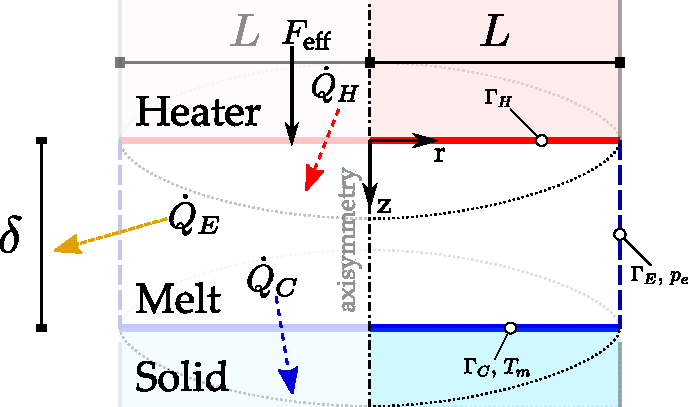
\includegraphics[trim=0 0 0 0 cm,clip,width=0.7\textwidth]{Chapters/Review/CCM/figs/cylindersketch/cylindersketch.pdf}
\caption[Close-Contact Melting: Problem Statement]{Problem description of a (cylindrical) close-contact melting problem. As heat is added through the heater surface $\Gamma_H$, a melt film of thickness $\delta$ separates the solid-liquid phase change interface (\gls{PCI}) $\Gamma_C$ from the heater. Note that the figure displays an axisymmetric cylindrical geometry with the axis of symmetry located at $r=0$. The symmetry is hinted at by the figure's brightness, the cylinder has the radius $L$. A constant pressure $p_e$ is assumed at the outflow boundary $\Gamma_E$. The simplified heat balance, sketched using the dashed arrows on the left half of the figure, distinguishes between a heat flux $\Dot{Q}_H$ induced by the heater, a heat flux $\Dot{Q}_C$ driving the phase change process and the outflux $\Dot{Q}_E$ leaving the system through the lateral outflow. \textit{Note that the Figure's aspect ratio is \textbf{not to scale} for better visibility.}} 
\label{fig:ccmsetupsketch}
\end{figure}


\subsubsection{Governing Equations in Cylindrical Coordinates}

While different phase change materials and heater geometries have been studied, all investigations rely on the common assumption that the film thickness $\delta$ is negligible compared to the heater's extensions in the other dimensions, e.g. $\delta \ll L$ or $\epsilon \coloneqq \delta / L\ll 1$ for the $2D$ case discussed here. In a Lagrangian frame of reference, tracking the interface (see Section \ref{fig:ccminterfacegeometry}), incompressible lubrication theory  \cite{hamrock2004fundamentalslubrication} then yields the following governing equations,
\begin{subequations}\label{eq:governingccm}
\begin{flalign}
    &\textit{Conservation of Mass}\quad && \frac{1}{r}\,\pdv{\qty(r\,u)}{r} + \pdv{w}{z}  = 0 & \quad , \label{eq:massccm}\\
    &\textit{Conservation of Momentum}\quad && \mu_L\,\pdv[2]{u}{z} = \pdv{p}{r} &   \quad ,\label{eq:momccm}\\
    &\textit{Conservation of Energy}\quad && u\,\pdv{T}{r} + w\,\pdv{T}{z}  = \alpha_L\,\pdv[2]{T}{z} & \quad , \label{eq:energyccm}
\end{flalign}
\end{subequations}

on the domain $\qty(r,\,z)\in\qty[-L,L]\cross\qty[0,\,\delta]$. This simplified set of equations is valid as long as the Reynolds number $\textit{Re}=\qty(\rho_L\,U\,L)/\qty(\epsilon\,\mu_L)$ satisfies $\textit{Re}\,\epsilon^2\ll1$. In the above equations $p$ and $T$ denote the pressure and temperature in the melt film. Variables $u,\,v$ denote $r$ and $z$-components of the velocity vector $(u,\,w)=(v_r,\,v_z) = \Vec{v}^T$. The material parameters $\mu_L$ and $\alpha_L=\kappa_L / \qty(\rho_L\,c_{p,L})$ are dynamic viscosity and thermal diffusivity respectively. $\kappa$ and $c_p$ refer to the material's thermal conductivity and specific heat capacity. Capital subscripts $L$ (\textit{liquid}), $S$ (\textit{solid}) and $G$ (\textit{gas}) will be used throughout this thesis to denote a parameters' phase affiliation.

The most important consequence of the scaling result \ref{eq:governingccm} is the depth independence of pressure $p$. It is preserved even in the compressible case (see Section \ref{sec:complubricationreview}).

\subsubsection{Boundary Conditions}

To solve the system of governing Equations \ref{eq:massccm}-\ref{eq:energyccm} we require boundary conditions for pressure $p$, temperature $T$, and velocity $\qty(u,w)$. 

Note that assuming a constant film thickness $\delta$ is a simplification to avoid further technicalities in the solution procedure, especially when it comes to a parametric description and numerical discretization of a domain with variable depth.  
Figure $\ref{fig:ccminterfacegeometry}$ sketches the interface geometry for a radially symmetric melt film of variable thickness. The center-line of symmetry is indicated by a gray vertical dash-dot line.

The surface normal is then given by

\begin{equation}
    \Vec{n} = \mqty(n_r \\ n_z) = \frac{1}{\sqrt{1 + \delta'(r)}}\mqty(\delta'(r) \\ -1) \quad ,
\end{equation}

For an in-depth derivation of governing equations given a variable melt film thickness and a discretization approach using a variable transformation the reader is referred to \cite{schuller2017spatially}. Throughout this thesis we will assume $\delta(r)\equiv \delta = \textit{const}$ or $\delta'=\partial\delta / \partial r = 0$, thus $n = n_z$. 

The boundary conditions for velocity then read
\begin{subequations}\label{eq:ccmvelocityboundary}
\begin{flalign}
     &\textit{Heater Surface} && u(r,0) = 0\,, \quad &w(r,0) &= 0\,, & \\
     &\textit{Interface Mass Conservation} && u(r,\delta) = 0\,, \quad & W \coloneqq w(r, \delta) &= -\frac{\rho_S}{\rho_L}\,U & \quad .
\end{flalign}
\end{subequations}

The interface boundary conditions ($z=\delta$) for velocity are based on the mass conservation condition across the interface discussed in Section \ref{sec:interfacedescription} and depend on the particular choice of a Lagrangian reference. Recalling the previous paragraph, the mass flow across the interface takes places in $z$-direction exclusively.

Temperature boundary conditions for a process driven by a surface heat flux $\Dot{Q}_H$ read
\begin{subequations}
\begin{flalign}
     &\textit{Fourier's Law} && \pdv{T}{z}\Bigg\rvert_{z=0} = -\frac{\Dot{Q}_H}{\kappa_L\,A\ts{h}} & \quad , \label{eq:ccmtempbcfluxheater}\\
     &\textit{Interface Melting Temperature} && T(x,\,z=\delta) = T_m  & \quad , \label{eq:ccmtempbcmeltingtemp}\\
     &\textit{Interface Stefan Condition} &&  \pdv{T}{z}\Bigg\rvert_{z=\delta} = - \frac{\rho_S\,U\,h_m^*}{k_L}  &\quad . \label{eq:ccmstefan}
\end{flalign}
\end{subequations}

On the interface the temperature field $T=T(r,\,z=\delta)$ has to satisfy melting temperature $T_m$. The equilibrium melting temperature is a point on the melting curve of the phase diagram (recall Fig. \ref{fig:phasediagram}) and, in principle, a function of the pressure $p(x)$ on the interface. However,  the temperature variation $T_m(p)$ is negligible for the pressure variations occurring in real \gls{CCM} melting scenarios and thus a constant Dirichlet boundary condition is imposed.

While the pressure distribution takes on a certain boundary pressure $p_e$ at the laterals,
\begin{equation}
    p(\pm L) = p_e\quad ,
\end{equation}

it only appears as a constant in the solution of Eqn. \ref{eq:momccm}. 



\begin{figure}[ht!]
\centering
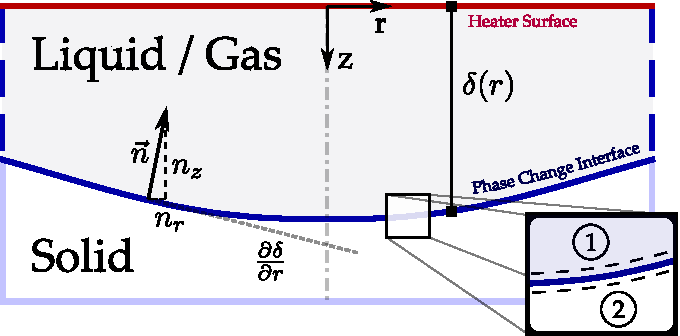
\includegraphics[trim=0 0 0 0 cm,clip,width=0.7\textwidth]{Chapters/Review/Interface/figs/interface/interfaceCylindrical.pdf}
\caption[Close-Contact Phase Change: Interface Description]{Variable thickness close-contact phase change problem. The figure illustrates the geometry of the interface parametrization $\delta(r)$ used in the description of (jump) boundary conditions on the phase change interface (\textit{solid, curved blue line}). The normal vector $\Vec{n}$ on the interface is of particular importance and sketched here at an arbitrary location on the \gls{PCI}. The direction of the surface tangent at the same position is given by $\partial\delta / \partial r$, hinted at by the dashed gray line. Note the assumed symmetry with respect to the $r=0$ center line (\textit{vertical dash-dot line}). For a given position on the interface we will formulate jump conditions in terms of the two phase's states $\mbox{\textcircled{\tiny 1}}$ and $\mbox{\textcircled{\tiny 2}}$ at infinitesimal distance from the \gls{PCI}.} 
\label{fig:ccminterfacegeometry}
\end{figure}

\subsubsection{Incompressible Solution}

The incompressible pressure profile for cylindrical close-contact can by found by algebraic manipulation of Eqns. \ref{eq:massccm}-\ref{eq:momccm} \cite{schuller2019icarus} and is given by relation 

\begin{equation}\label{eq:pincompcylinder}
    p(r) = p_e + \frac{3\,\mu_L\,W\,\qty(L^2-r^2)}{\delta^3} \quad \quad r \in \qty[-L,L] \quad ,
\end{equation}

with (constant) interface fluid velocity $W$ related to the Stefan velocity $U$ by $W = \qty(\rho_S / \rho_L)\, U$ (Eqn. \ref{eq:ccmvelocityboundary}). 

The horizontal and vertical velocity components $u$ and $w$ are then found from
\begin{subequations}\label{eq:incompccmvelocity}
\begin{flalign} 
    \qquad \qquad & u(r,z) = -\frac{6\,r\,\mu_L\,W\,r\,z\,\qty(z-\delta)}{\delta^3} & \quad \qty(r,\,z)\in \qty[-L,\,L]\cross\qty[0,\,\delta] \quad ,\\
    \qquad \qquad &  w(r,z) = \frac{6\,W}{\delta^3}\,\qty(\frac{z^3}{3} - \frac{z^2}{2}\,\delta) & \quad \qty(r,\,z)\in \qty[-L,\,L]\cross\qty[0,\,\delta] \quad .
\end{flalign}
\end{subequations}

% \begin{equation} \label{eq:incompressibleheat}
%     \rho_L\,c_{p,L} \, \qty(u\,\pdv{T}{x} + w\,\pdv{T}{z}) = \kappa_L \, \pdv[2]{T}{z} \quad \quad \quad\quad \qty(r,\,z)\in \qty[-L,\,L]\cross\qty[0,\,\delta] 
% \end{equation}

Instead of numerically solving the incompressible heat Equation \ref{eq:energyccm} across the melt, the authors of \cite{schuller2019icarus} propose to prescribe a quadractic $1D$ polynomial that satisfies the heating flux boundary condition at $z=0$ (Eqn. \ref{eq:ccmtempbcfluxheater}) and the melting temperature and Stefan condition on the \gls{PCI}, $z=\delta$ (Eqns. \ref{eq:ccmtempbcmeltingtemp} and \ref{eq:ccmstefan}). Using the three boundary conditions to solve for the polynomial's coefficients one obtains 
\begin{equation}\label{eq:temperaturequadraticreview}
    T(r,z) = \frac{\Dot{q}_H - \rho_S\,U\,h_m^*}{2\,\delta\,\kappa_L}\,\qty(z^2-\delta^2) + \frac{\Dot{q}_H}{\kappa_L}\,\qty(\delta - z) + T_m \quad .
\end{equation}

Here we introduced $\Dot{q}$ as our notation for the heat flux in $\Dot{q}_H=\Dot{Q}_H / A_H$, where $\Dot{Q}_H$ is the power added to the system through the heater surface ($z=0$) of area $A_H$.
As shown in the later Chapter \ref{chap:results}, Ansatz \ref{eq:temperaturequadraticreview} can indeed be validated to be an accurate approximation to the real solution of Eqn. \ref{eq:energyccm} in incompressible melting. It is however not directly clear if this result generalizes to compressible flows. 

The cylindrical contact force is readily computed by integrating the pressure over the heater surface
\begin{equation}\label{eq:ccmpressureforce}
    F_p = 2\,\pi\,\int_0^L \qty(p(\hat{r})-p_e)\,\hat{r}\, \mathrm{d}\hat{r} \quad .
\end{equation}

To evaluate Eqns. \ref{eq:incompccmvelocity} and \ref{eq:temperaturequadraticreview} one requires knowledge about the melt film thickness $\delta$. A closure relation proposed in \cite{schuller2019icarus} uses the fact that the correct equilibrium melt film thickness $\delta$ must be found such that 
\begin{enumerate}

    \item the temperature $T(r, z)$ satisfies the Stefan condition (Eqn. \ref{eq:ccmstefan}) everywhere on the interface $z=\delta$ (\textit{thermodynamic equilbrium)} and
    \item the contact force $F_p$ (Eqn. \ref{eq:ccmpressureforce}) exerted by the pressure  distribution is in balance with the effective force $F\ts{eff}$ induced by the melting probe (\textit{mechanical equilibrium}).  
\end{enumerate}

The two conditions can be used to find two independent relations for $\delta$,
\begin{subequations}
\begin{flalign}
     & \textit{from thermodynamic equilbrium } && \delta= \frac{20\,\alpha_L\,\rho_L\qty(\Dot{q}_H-\rho_S\,U\,h_m^*)}{U\,\rho_S\,\qty(3\,\Dot{q}_H + 7\,\rho_S\,U\,h_m^*)} & \quad , \label{eq:ccmdeltathermodynamic}\\
     & \textit{from mechanical equilbrium } && \delta= \qty(\frac{3}{2}\,\frac{\pi\,L^4\,\mu_L\,\frac{\rho_S}{\rho_L}\,U}{F_p - \rho_L\,V\ts{probe}\,g})^{1/3}& \quad .
\end{flalign}
\end{subequations}

The correct equilibrium melt film thickness can be found by equating the two relations above and solving for $\delta$ using a numerical root finding strategy.

In  Table \ref{tab:ccmequilibria} we summarize the role of equilibrium conditions as convergence criteria in iterative solvers for the state of an equilibrium close-contact phase change system. 
Note that this is assuming an effective force $F\ts{eff}$ as an input to the system. One can also just assume a velocity $U$. The resulting pressure distribution $p$ can then be integrated (Eqn. \ref{eq:ccmpressureforce}) to find the required force $F\ts{eff}$ to achieve a given $U$. 

\begin{table}[ht!]
\begin{tabular}{ll|
>{\columncolor[HTML]{EFEFEF}}l |l|
>{\columncolor[HTML]{ECF4FF}}l}
\textit{Equilibrium Cond.}                                                      &  & \textbf{Thermodynamical (a)}                                                              &  & {\color[HTML]{333333} \textbf{Mechanical (b)}}                                                                       \\
\textit{Iteration Variable}                                                    &  & \begin{tabular}[t]{@{}l@{}}Lubrication Film Thickness\\ $\delta$\end{tabular}  &  & {\color[HTML]{333333} \begin{tabular}[t]{@{}l@{}}Interface Prop. Speed\\ (\textit{Stefan Velocity}) $U$\end{tabular}}                         \\
                                                                               &  &                                                                                                  &  &                                                                                                       \\
\textit{\begin{tabular}[t]{@{}l@{}}Coressponding Flow\\ Property\end{tabular}} &  & \begin{tabular}[t]{@{}l@{}}Steady Temperature\\ Distribution $T(x,z)$\end{tabular}    &  & {\color[HTML]{333333} \begin{tabular}[t]{@{}l@{}}Pressure Distribution $p(x)$\\ \end{tabular}}                    \\
                                                                               &  &                                                                                                  &  &                                                                                                       \\
\textit{Macroscopic Balance}                                                   &  & \begin{tabular}[t]{@{}l@{}}Local Energy Conservation \\ at the Interface \\ (\textit{Stefan Condition}
)\end{tabular}                                                            &  & {\color[HTML]{333333} \begin{tabular}[t]{@{}l@{}}Effective Force $F\ts{eff}$\\ \end{tabular}}
\end{tabular}
\caption[Equilibrium in Close-Contact Phase Change]{Mechanical and thermal balance in close-contact phase change. Close-contact models aim to find the state of system at which (\textbf{a}) the temperature distribution satisfies the interface \textit{Stefan condition} (Eqn. \ref{eq:stefancondition}) and (\textbf{b}) the pressure distribution $p(x)$ is in balance with the effective force $F\ts{eff}$ (Eqn. \ref{eq:feffective}) exerted on the lubrication film (\textit{mechanical equilibrium}). The film thickness $\delta$ and Stefan velocity $U$ can be iterated upon, to match conditions \textbf{(a)} and \textbf{(b)} respectively.}
\label{tab:ccmequilibria}
\end{table}


\subsubsection{Energy Balance and Melting Efficiency}\label{subsec:ccmefficiency}

Following \cite{schuller2019icarus}, a very basic melt film energy balance distinguishes between three contributions
\begin{equation}
    \Dot{Q}_H - \Dot{Q}_E - \Dot{Q}_E = 0 \quad .
\end{equation}

The power $\Dot{Q}_H$ is added trough the heater surface $\Gamma_H$ with area $A_H$. This heat is split among the heat flux across the \gls{PCI}, $\Dot{q}_C=\Dot{Q}_C / A_H$, which is necessary to sustain phase change, and a loss $\Dot{q}_E$ through the lateral outflow boundary $\Gamma_E$. The control domain and the heat flow are sketched in Fig. \ref{fig:ccmsetupsketch}.

As a measure of process efficiency $\gamma$ one can now define the fraction
\begin{equation}\label{eq:defgamma}
    \gamma \coloneqq \frac{\Dot{Q}_C}{\Dot{Q}_H} = \frac{\Dot{q}_C}{\Dot{q}_H}
\end{equation}

of the total input heat used to drive the phase change process. In the limit of perfect efficiency, $\gamma = 1$, we have $\Dot{q}_C = \Dot{q}_H$ or $\Dot{q}_e = 0$, meaning that the full heating power is used to melt the ice and no convective losses occur.

The Stefan condition at the \gls{PCI} lets us rewrite Eqn. \ref{eq:defgamma} in terms of the effective Stefan velocity $U$ of the melting process. 

\begin{framed}
Recalling the Stefan condition $\Dot{q}_C = \rho_S\,U\,h_m^*$, we find an upper limit $U^*$ for the Stefan velocity at optimal efficiency ($\gamma = 1$) from
\begin{equation}\notag
     \Dot{q}_C^*  =  \rho_S\,U^*\,h_m^* \overset{\gamma = 1}{=} \Dot{q}_H \quad
    \Longleftrightarrow\quad   U^*=  \frac{\Dot{q}_H}{ \rho_S\,h_m^*}\notag \quad ,
\end{equation}
allowing us to rewrite the efficiency in terms of the velocity ratio
\begin{equation}
    \gamma = \frac{\Dot{q}_C}{\Dot{q}_H} = \frac{U}{U^*} \quad .
\end{equation}

In this context, the ideal Stefan velocity $U^*$ is understood as theoretical limit for the achievable interface propagation speed at a given input heat flux $\Dot{q}_H$.
\end{framed}

The efficiency $\gamma$ can be used to gain an intuition for the behavior of close-contact phase change. A high efficiency, in the sense that most energy supplied by the heating device is used to drive the phase change process ($\gamma\approx 1$), can be achieved by increasing the effective force $F\ts{eff}$ exerted by the melting probe. This is possible by increasing its weight or by means of a screw \cite{dachwald2014icemole}.

We will later discuss the role of $\gamma$ as a similarity parameter in the gas temperature solution of equilibrium sublimation states.



\FloatBarrier